\documentclass[10pt]{article}

\usepackage{graphicx}
\usepackage{amsmath}
\usepackage{amssymb}
\usepackage{braket}
\usepackage{parskip}
\graphicspath{{../../figs/}}

\begin{document}

\title{Hiddem Markov Models for protein dynamics}

\section{Motivation}

Traditionally, we have clustered conformation-space into many discrete
voronoi cells and used this clustering to build a large transition matrix.
This results in implied timescales that are consistently faster than they
should be. 

The motivation of this work can be found in considering a simple, two-well,
1D potential. What is the optimal clustering? There are only two physically
stable states, but if we used two \textit{hard} states, conformations on the cusp
of the barrier are considered to be the same as conformations at the bottom of the well.
If the particle moving under this potential diffuses for a bit at the top of the potential,
crossing the line that distinguishes our two hard states, it generates many counts, distorting
the dynamics. 

The theoretical underpinnings of Markov State Models is that they are used to estimate
the propagator. The true propagator is continuous in $\mathbb{R}^{6N}$, and the typical
approach is to use indicator basis functions to approximate it. This gives step-like
eigenfunctions whose resolution increases with increasing number of states. One can imagine
using a different basis set instead. Two Gaussian functions, for example, could describe
dynamics on this potential much better than even a high number of step functions.

Deriving a transition matrix from non-overlapping hard states is trivial: for lag time
$\tau$, if the conformation moves from state $i$ to state $j$ increment the entry
in the count matrix, $C_{ij}$. The transition matrix is a row-stochastic version of
this count matrix.

It is impossible to define counts in this way for \textit{fuzzy} states. One might
imagine describing a point at time $t$ not simply as belonging to state $i$, but rather as 
having a vector of memberships $\mathbf{m}$ in each fuzzy state. One might think
that you can get the transition matrix by summing the outer product between each
time-pair of membership vectors as in REF

\begin{equation}
\sum \Ket{\mathbf{m}_t} \Bra{\mathbf{m}_{t+1}}
\end{equation}

This works for the case of quantized memberships, but creates
arbitrarily small transition probabilities due to the multiplication
of many numbers that are less than one. In fact, the problem
of coming up with a transition matrix from fuzzy states is non-trivial.
Going back to our two well potential, consider a conformation sitting at
the top of the barrier. It has membership vector $\mathbf{m}_0 = (0.5,0.5)$. 
After one time step, it is in the same place, $\mathbf{m}_1 =(0.5, 0.5)$

\begin{figure}[h!]
	\centering
	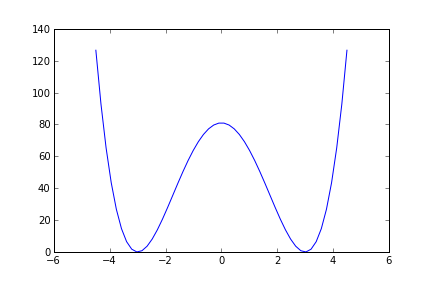
\includegraphics[width=0.5\textwidth]{two-well.png}
	\caption{two well potential}
\end{figure}

\section{two}

\end{document}